% file: 01-pattern-even-cases.tex

\documentclass[tikz]{standalone}
\usetikzlibrary{decorations.pathreplacing, positioning, arrows.meta, shapes.multipart, calc}

\begin{document}
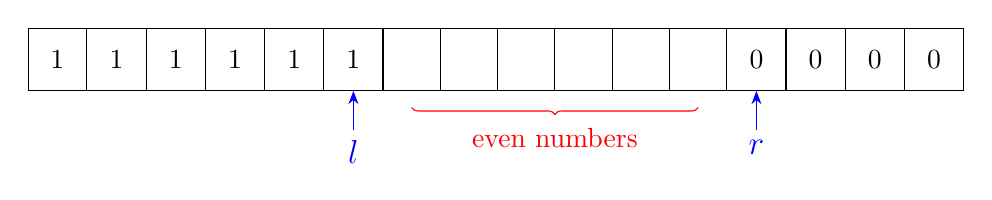
\begin{tikzpicture}[Array/.style = {rectangle split, rectangle split parts = #1, rectangle split horizontal,
    inner sep = 8pt, anchor = center}]
    % bit array

    % index
    \node[Array = {16}, draw] (A) 
      {1\nodepart{two}1\nodepart{three}1\nodepart{four}1\nodepart{five}1\nodepart{six}1
       \nodepart{seven}\nodepart{eight}\nodepart{nine}\nodepart{ten}\nodepart{eleven}\nodepart{twelve}
       \nodepart{thirteen}0\nodepart{fourteen}0\nodepart{fifteen}0\nodepart{sixteen}0};

   \node (l) [below = 0.5cm of A.six south, font = \large, blue] {$l$};
   \draw[->, >=Stealth, blue] (l) to (A.six south);

   \node (r) [below = 0.5cm of A.thirteen south, font = \large, blue] {$r$};
   \draw[->, >=Stealth, blue] (r) to (A.thirteen south);

   \draw[decoration = {brace, mirror, raise = 6pt}, decorate, red] (A.seven south) -- node[below = 10pt, align = center] 
	{even numbers} (A.twelve south);
\end{tikzpicture}
\end{document}

